\documentclass[10pt,a4paper]{report}
\usepackage[english]{babel}
\usepackage{amsmath}
\usepackage{graphicx}
\usepackage{lmodern}
\usepackage[font=small,format=plain,labelfont=bf,up,textfont=it,up]{caption}
\usepackage[nottoc]{tocbibind}
\usepackage{url}
\usepackage{courier}
\usepackage[T1]{fontenc}
\usepackage[titles]{tocloft}
\usepackage{subcaption}
\usepackage{listings}
\usepackage{color}
\usepackage{algorithm}
\usepackage{algpseudocode}

\setcounter{secnumdepth}{5}
\setlength{\parindent}{0in}

\renewcommand{\topfraction}{0.85}
\renewcommand{\textfraction}{0.1}
\renewcommand{\floatpagefraction}{0.75}
\definecolor{dkgreen}{rgb}{0,0.6,0}
\definecolor{gray}{rgb}{0.5,0.5,0.5}
\definecolor{mauve}{rgb}{0.58,0,0.82}
\definecolor{darkred}{rgb}{0.9,0,0}

\lstset{frame=tb,
  language=C++,
  aboveskip=5mm,
  belowskip=5mm,
  showstringspaces=false,
  columns=flexible,
  basicstyle={\small\ttfamily},
  numbers=none,
  numberstyle=\tiny\color{gray},
  keywordstyle=\color{blue},
  commentstyle=\color{dkgreen},
  stringstyle=\color{mauve},
  breaklines=true,
  moredelim=**[is][\color{darkred}]{@}{@},
  breakatwhitespace=true,
  tabsize=3
}

\newcounter{example}
\newcounter{algorithmCode}

\makeatletter
\lstnewenvironment{example}[2]{
  \renewcommand\lstlistingname{Example}
  \let\c@lstlisting=\c@example
  \let\thelstlisting=\theexample
  \lstset{caption=#1, label=#2}
} {}

\lstnewenvironment{algorithmCode}[2]{
  \renewcommand\lstlistingname{Algorithm}
  \let\c@lstlisting=\c@algorithmCode
  \let\thelstlisting=\thealgorithmCode
  \lstset{caption=#1, label=#2}
} {}
\makeatother

\makeatletter
\newcommand\ackname{Acknowledgements}
\if@titlepage
  \newenvironment{acknowledgements}{
      \titlepage
      \null\vfil
      \@beginparpenalty\@lowpenalty
      \begin{center}%
        \bfseries \ackname
        \@endparpenalty\@M
      \end{center}}%
     {\par\vfil\null\endtitlepage}
\else
  \newenvironment{acknowledgements}{
      \if@twocolumn
        \section*{\abstractname}
      \else
        \small
        \begin{center}
          {\bfseries \ackname\vspace{-.5em}\vspace{\z@}}
        \end{center}
        \quotation
      \fi}
      {\if@twocolumn\else\endquotation\fi}
\fi
\makeatother

\title{CuEira, Gene-Environment Interaction Analysis on GPU}
\author{Daniel Berglund}
\date{October 2014}

\begin{document}
\maketitle
\thispagestyle{empty}

\clearpage
\thispagestyle{empty}
\selectlanguage{english}
\begin{abstract}
Abstract in english
\end{abstract}

\clearpage
\thispagestyle{empty}
\selectlanguage{english}
\begin{abstract}
Abstract på svenska
\end{abstract}

\clearpage
\thispagestyle{empty}
\begin{acknowledgements}
Asdf
\end{acknowledgements}

\clearpage
\tableofcontents
\thispagestyle{empty}

\clearpage
\setcounter{page}{1}
\chapter{Introduction}

\section{Outline}
The first chapter contains an short introduction to the area and some termonology.

Appendix has list of variables and acronyms

\section{Genetics}
Some kind of intro\\
\\
The DNA is spread over chromosomes, each chromosome comes in a pair that can have different variations in them. A position in the DNA is a locus. An variation of the same gene or locus is an allele. The effect of an allele is either dominant, recessive or co-dominant. Dominant means that the effect occurs if the allele only needs to be present once to get the effect, recessive is when the allele has to be in both chromosomes. Co-dominant is when both alleles are expressed, this usually produce some kind of intermediate state.\cite{sadava_life}\\
\\
4 bases\cite{sadava_life}\\
\\
SNPs are variations in the genome where a single nucleotide is different between individuals in a population\cite{fareed_snp}

\section{Genome-wide association studies}
One type of study to find links between genetic markers and diseases is genome-wide association studies(GWAS). The markers are usually the SNPs mentioned above. Classically GWAS does not consider interactions between the genetic markers or with environmental factors. The environmental factors can be various things such as smoking, physical activity and so on.  Investigating gene-gene interactions recently has become more common\cite{cordell_detect_review}, however gene-environment interactions are still an uncommon in studies\cite{gene_enviroment_2013}. Interactions between genes and environmental factors are considered to be important for complex diseases such as cancer and autoimmune diseases\cite{cordell_detect_review, gene_enviroment_2013, geira, ra_smoking}. A complex disease develops due to a combination of factors, not a single gene or environmental factor\cite{rothman1998modern}.\\
\\
GWAS usually have either cohort or case-control study design. In cohort study a sample of a population is followed and over time some individuals will develop the disease of interest. In case-control studies two groups are compared with each other to find risk factors. One group consists of individuals with the disease and the other of individuals that are similar to the cases but who do not have the disease.\cite{rothman1998modern,mann_observational}\\
\\
A typical study consists of tens of thousands of individuals and hundred thousands or millions of SNPs. Due to the high number of SNPs few algorithms are capable to investigate more than second order interaction in a reasonable time. There are some algorithms that can handle higher interaction orders however these have drawbacks\cite{gwis,high_order_2012,fast_high_order_cluster}.

\section{Defining Interaction}
There are several ways to define interaction. The overall goal is usually to detect if \emph{biological} interactions are present. \emph{Biological} interaction is when the factors co-operate through a physiological or biological mechanism and causes the effect, e.g. the disease. This information can be used to explain the mechanisms involved in causing the disease and possibly help to find cures for them. However biological interaction is not well defined and thus it is not possible to calculate it directly from data.\cite{rothman1998modern,rothman2002intro_epidemiology}\\
\\
\emph{Statistical} interaction on the other hand is well defined. However it is scale dependent, i.e. interactions can appear and disappear based on transformations of the data. Statistical interaction also depends on the model used. The common way to define statistical interaction is to consider the presence of a product term between the variables in the statistical model, this is referred to as \emph{multiplicative} interaction. For instance for a linear model
\begin{equation}
f(x,y)=ax+by+cxy+d
\end{equation}
$c$ is the product term that represents multiplicative interaction between variables x and y. Statistical interaction is often referred to as just interaction which can make it a bit confusing.\cite{geira,rothman1998modern}\\
\\
\emph{Additive} interaction is a bit broader than multiplicative interaction. It is that the effect from the interaction is larger than the sum of the separate effects. It implies biological interaction as defined by Rothman, which is sometimes called \emph{causal interdependence} or \emph{causal interaction}. A more precise definition can be found in section \ref{additive}

\section{GEIRA and JEIRA}
\label{jeira}
\emph{GEIRA} is a tool for analysing gene-environment interaction. It uses logistic regression and causal interaction\cite{geira}. \emph{JEIRA} is a parallelised implementation of GEIRA\cite{uvehag_master_thesis}.

%TODO something about GEISA
%TODO graph or such of development?

\section{Aim of Project}
The aim of this project was to build a program for gene-environment using logistic regression and utilizing graphic cards to speed up the calculations.

\clearpage
\chapter{Background}
%TODO
Intro here\\
\\
Most of the conducted research on interactions in GWAS has been focused on gene-gene interactions. Few studies and tools have been investigating gene-environment interactions.

Both CPU clusters\cite{biforce} and GPUs\cite{gwis,gboost,gmdr_gpu,cuda_lr,genie_2012,plink_gpu} have been used for GWAS. GPUs have been a popular choice since most of the methods for searching for interaction are good on GPUs because each combination of variables can commonly be considered independently from the others. More about this in section \ref{gpu_gwas}

%Bla bla lite om outline

\section{Minor Allele Frequency and Risk Allele}
%TODO +vart placera?
An allele itself doesn't contain the information if it is harmful or not so to

The \emph{risk allele} is


SNPs are commonly binary variables with either dominant or recessive models. The case where the risk would occur given the genetic model is coded as 1 and absence is coded as 0. Co-dominant model can also be used and in that case when an individual has the risk allele in both positions is coded as 2, when only one is present is coded as 1 and absence is 0 as before. The fact that it's a binary variable is used in a lot of algorithms because it simplifies things.\\



\emph{Minor allele frequency}(MAF) is the frequency of the least common allele. If it is too low an analysis will be of little value, 5\% is usually used as the threshold. The same problem occurs if the absolute number is too low.

\section{Algorithmic Background}
%TODO bit better intro
This section will introduce the statistics and some of the algorithms used to search for interaction. The focus is on logistic regression but some other methods are briefly examined.\\
\\
There are a lot of algorithms and programs proposed for searching for interaction, most have focused on gene-gene interaction as already mentioned. They can be roughly classified into four categories, exhaustive, stochastic, machine learning/data mining and stepwise\cite{fast_high_order_cluster}.	\\
\\
Environmental factors can be of any variable type(i.e. binary, continuous, categorical) which creates problems in various ways\cite{gene_enviroment_2013}. Gene-gene interaction tools can sometimes be used to find gene-environment interaction, however they usually require the variables to be binary or have other problems since they weren't designed for environmental interaction.\cite{gene_enviroment_2013}\\
\\
\emph{Exhaustive search} is the most direct approach, it compares all combinations of the SNPs in the dataset. Exhaustive search methods will not miss a significant combination because it didn't consider that specific combination. However it also means that they can be slow since they will spend time on combinations other methods would skip completely. Multifactor-Dimensionality Reduction(MDR)\cite{mdr_2001} and BOOST\cite{boost_gene_gene} are two examples of this type of algorithm.\\
\\
\emph{Stochastic} methods uses random sampling to iterate through the data. BEAM\cite{beam_2007} is one example and it uses Markov Chain Monte Carlo(MCMC) method.\\
\\
\emph{Data Mining} and \emph{Machine Learning} are methods that try to learn patterns from data and tries to generalize it. MDR\cite{mdr_2001} is a type of data mining method and is among the most common methods used in GWAS. See section \ref{data_machine_learning} for more details.\\
\\
\emph{Stepwise} methods uses a filtering stage and a search stage. At the filtering stage uninteresting combinations are filtered out by using some exhaustive method. The other SNPs are the examined more carefully in the search stage. BOOST\cite{boost_gene_gene} is an example which uses succinct data structures and a likelihood ratio test to filter the data before applying log-linear models.

\subsection{Confounders and Covariates}
\emph{Confounding} is one of the central issues in design of epidemiological studies. It is when the effect of the exposure is mixed with the effect of another variable. So if we do not measure the second variable, the effect of the first would be estimated as stronger than it really is. The second variable is then a \emph{confounder}. Several methods in epidemiology are about avoiding or adjusting for confounding. Sometimes these variables needs to be incorporated into the models. \emph{Covariates} are possible confounders or other variables that one wants to adjust for in the model. Sometimes covariates are called \emph{control variables}.\cite{rothman2002intro_epidemiology,rothman1998modern}

\begin{figure}[h]
    \centering
    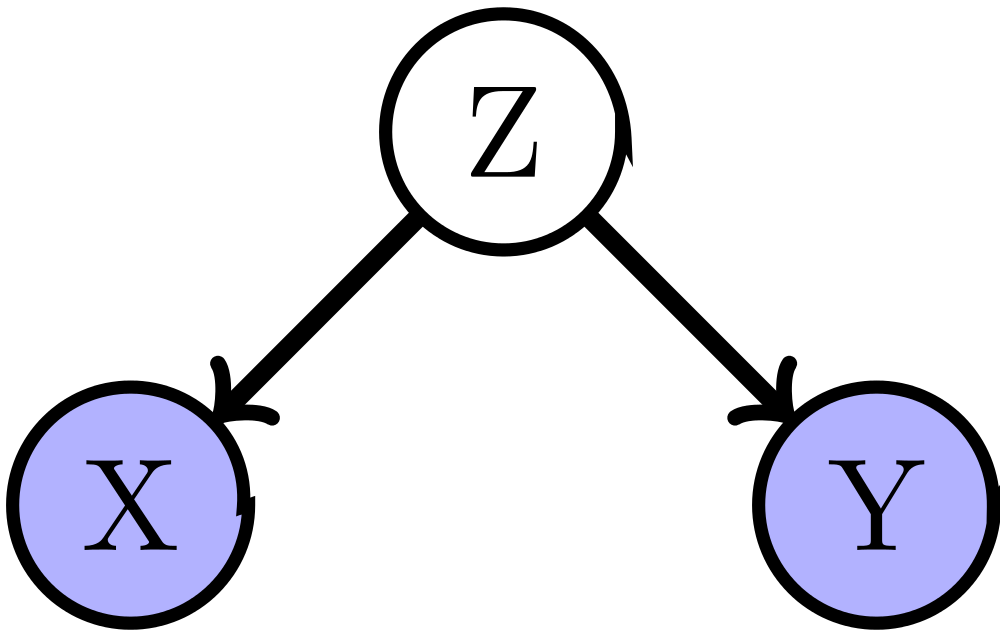
\includegraphics[width=5cm]{Simple_Confounding_Case.png}
    \caption{Illustration of a simple case of confounding. If we do not observe Z we might falsely find an association between X and Y}
    \label{fig:confunding}
\end{figure}

For instance if a study would look into the effects of yellow teeth on lung cancer they would likely find an effect. However it would be due to the confounder smoking since smoking causes yellow teeth and lung cancer. %TODO cite

\subsection{The Multiple Testing Problem}
It is not uncommon to test a lot of hypothesis on the same data and in the case of GWAS it can be billions of tests. If one continues to test one should eventually find something that is significant due to random chance. With the common significance threshold of 5\% it is expected to get 1 in 20 false positives under the assumption that the null hypothesis is true. The problem arises from the fact that the hypothesis tests are dependent on each other since they use parts of the same data. This is the multiple testing problem and if it is not corrected for a lot false positives might be found.\cite{bonferroni_multiple}\\
\\
Bonferroni correction is the simplest method and viewed as a conservative way to correct for this problem. It simply divides the significance threshold by the number of hypothesis tested. However the number of hypothesis made is not always clear. With a two-stage analysis, is the number of hypothesis the number of tests done in both stages combined, the number made in the first stage or the second stage?\cite{bonferroni_multiple}

\subsection{Contingency Tables}
A contingency table is a matrix used to describe categorical data. Each cell contains a count of occurrences for a specific combination of variables. Table \ref{table:contingency_table} is an example of an 2 x 2 table. From this table we can for instance see that 688 smokers got lung cancer. Contingency tables are the basis for various statistical tests to model the data.\cite{agresti_categorical}

\begin{table}[h]
\begin{tabular}{| l c c |}
  \hline
  & Lung cancer & No lung cancer\\
  \hline
  Smoker & 688 & 650 \\
  Non smoker & 21 & 59 \\
  \hline  
\end{tabular}
\caption{Contingency table describing the outcome of a study, from \cite{agresti_categorical}, page 42}
\label{table:contingency_table}
\end{table}

\subsubsection{Relative Risk and Odds Ratio}
From a contingency table it is possible to calculate some useful measures such as the risk of getting the outcome based on exposure. The risk for a row $i$ in the table will be referred to as $\pi_i$. For table \ref{table:contingency_table} the risks $\pi_1$ and $\pi_2$ is

\begin{equation}
\pi_1=\frac{688}{688+650}=0.51
\end{equation}

\begin{equation}
\pi_2=\frac{21}{21+59}=0.36
\end{equation}

To compare different risks, for instance between smokers and non smokers, the ratio of the risks is used\cite{agresti_categorical}. It is called \emph{relative} risk(RR) is defined as\cite{agresti_categorical} 

\begin{equation}
RR=\frac{\pi_1}{\pi_2}
\end{equation}

So for the table \ref{table:contingency_table} the relative risk of getting lung cancer based on exposure to smoking is

\begin{equation}
RR=\frac{0.52}{0.36}=1.96
\end{equation}

This means that the risk of getting lung cancer for a smoker is almost twice as high for a non smoker in this data.\\
\\
Another useful measure is \emph{odds} and \emph{odds ratio}(OR). The odds is\cite{agresti_categorical} 

\begin{equation}\label{eq:odds}
\Omega=\frac{\pi}{1-\pi}
\end{equation}

The odds are non-negative and $\Omega>1$ when the outcome is more likely than not\cite{agresti_categorical}. So for $\pi=0.75$ the odds is $\Omega=\frac{0.75}{1-0.75}=3$. This means that the outcome is 3 times more likely to occur than not. ORs can be used as an approximation of RR in case control studies because RR can not be estimated in that type of studies\cite{or_mislead}. Cohort studies on the other hand can give estimates of RR. FIXME cite\cite{}. OR is the ratio of the odds just as RR is the ratio of the risks\cite{agresti_categorical}.

\begin{equation}\label{eq:odds_ratio}
\theta=\frac{\Omega_1}{\Omega_2}
\end{equation}

In the case when the outcome is a disease or similar variables with odds ratio below one are called \emph{protective} and when it is above one it is a \emph{risk factor}\cite{recoding_2011}.

\subsection{Logistic Regression}
One way to model the contingency tables is by using \emph{logistic regression}. Logistic regression is a type of linear regression model for classification that models a latent probability for the outcomes. The outcomes are binary, however the method can be extended to multiple outcomes. In this work we will only consider them as binary. Logistic regression transforms the probability by using the \emph{logit} transformation. The logit transformation with probability $\pi$ is \cite{agresti_categorical}

\begin{equation}\label{eq:logit}
log(\frac{\pi}{1-\pi})
\end{equation}

\begin{figure}[h]
    \centering
    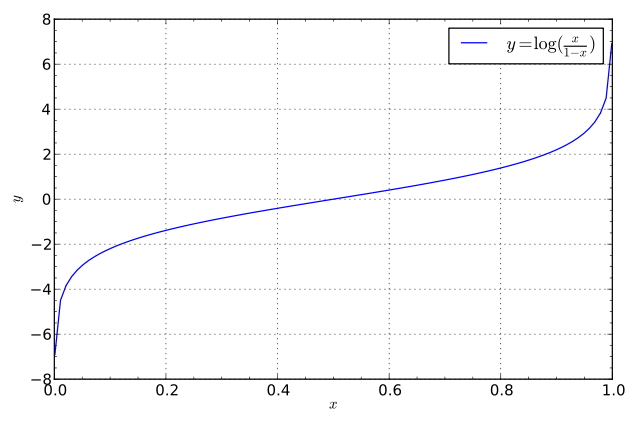
\includegraphics[width=7cm]{logit.png}
    \caption{Graph of the logit transformation. Wikipedia Commons}
    \label{fig:logit}
\end{figure}

The probability with a set of predictor variables \emph{X} is $\pi(X)=P(Y=1)$. The linear regression model with n predictors $X=(x_1,x_2,....,x_n)$, coefficients $\beta=(\beta_1, \beta_2,....,\beta_n)$ and by using the logit transformation is then\cite{agresti_categorical}
\begin{equation}\label{eq:logit_lr}
logit[\pi(X)]=\alpha+\beta X
\end{equation}

By moving the logit to the right side of the equation we get the model of the probability\cite{agresti_categorical}
\begin{equation}
\pi(X)=\frac{e^{\alpha+\beta X}}{1+e^{\alpha+\beta X}}
\end{equation}

The logit, equation \ref{eq:logit}, also happens to be the log of the odds(equation \ref{eq:odds})\cite{agresti_categorical}. By exponentiating both sides of equation \ref{eq:logit_lr} it shows that the odds is \cite{agresti_categorical}

\begin{equation}
e^{logit[\pi(X)]}=\frac{\pi(X)}{1-\pi(X)}=e^{\alpha+\beta X}=\Omega
\end{equation}

This means that $\exp{\beta}$ is the odds ratio since the odds increase by $\exp{\beta}$ for each unit increase of $X$\cite{agresti_categorical}. It can also been seen by taking the ratio of the odds using equation \ref{eq:odds_ratio} and  with $X=x+1$ and $X=x$

\begin{equation}
\theta=\frac{e^{\alpha+\beta (x+1)}}{e^{\alpha+\beta x}}=e^{\alpha+\beta (x+1)-\alpha-\beta x}=e^{\beta}
\end{equation}

Finding the $\beta$ coefficients are done in a similar way as with other linear regression models since they all are generalized linear models \cite{agresti_categorical}. It's usually done using  maximum likelihood(ML), via Newtons method\cite{agresti_categorical, uvehag_master_thesis}. It's an iterative method which means it can be relatively slow compared to non iterative methods. Below is pseudo code for the algorithm using Newtons method\cite{uvehag_master_thesis}.\\
\\
Fix this part a bit %TODO
Note: $\cdot$ is matrix-matrix or vector, * is element by element\\
X is the variables(N X M), Y outcomes with length N, beta is length M
M=number of predictors excluding intercept
result beta is M+1

%TODO label and caption
\begin{algorithm}
\begin{algorithmic}
\State $\boldsymbol{X}\gets
\begin{pmatrix}
\begin{matrix}
  1\\
  \vdots\\
  1
\end{matrix} & \boldsymbol{X}
\end{pmatrix}
$

\State $\beta\gets
\begin{pmatrix}
  0\\
  \beta
\end{pmatrix}
$

\State $iter\gets 0$
\State $diff\gets 1$
\\
\While{$iter < max\_iter \; \boldsymbol{and} \; diff > threshold$}
\State $\beta_{old}\gets\beta$
\State $p\gets \frac{e^{\boldsymbol{X} \cdot \beta}}{1+e^{\boldsymbol{X} \cdot \beta}}$
\State $s\gets \boldsymbol{X^T}\cdot (\boldsymbol{Y}-p)$
\State $\boldsymbol{J}\gets (\boldsymbol{X^T}\cdot (p*(1-p)))\cdot \boldsymbol{X}$
\State $\beta\gets \beta_{old}+\boldsymbol{J}^{-1} \cdot s$
\State $diff\gets \sum |\beta-\beta_{old}|$
\State $iter\gets iter+1$
\EndWhile
\State $log \; likelihood\gets \sum (\boldsymbol{Y}*ln p+(1-\boldsymbol{Y})*ln(1-p))$
\end{algorithmic}
\end{algorithm}

\subsubsection{Mathematical Definition of Interaction for LR}
\label{additive}
The more precise defintion of additive interaction is, the divergence from additive effects on a logarithmic scale, e.g.

\begin{equation}
OR_{both\:factors\:present}>OR_{first\:factor\:present}+OR_{second\:factor\:present}-1
\end{equation}

\cite{rothman1998modern}

The interaction variable needs to be represented and this is done by looking at how the model looks.

%math stuff for mult

%math stuff for add

However there is a problem when both variables are non binary. Because LR models how the risk increases for each increase in the variable the interaction variable should preferably be in increased order of risk. However without doing extensive testing for the possible combinations it is not possible to know the order. It is easy in the binary case because the interaction only has two levels, both present or not. For an example take two variables with 3 levels, 0,1,2. For a single variable it is easy to assume that 2 is worse than 1. The problem with interaction occurs here because it is hard to know if 1,2 is worse than 2,1. In the case of continues variables it gets worse because scale starts to matter more.

However in gene-environment interaction the SNP variable is binary unless co-dominant model is used. This means that the coding isn't a problem for non binary environmental variables.


Extending to non binary.

\begin{equation}
OR_{both\:factors\:present}^x>OR_{first\:factor\:present}+OR_{second\:factor\:present}^x-1
\end{equation}
Where x is the number of steps from the base level.

This means that the interaction depends on the level of the factor. There are four cases

Using $\beta_{snp}$
$\beta_{environment}$
$\beta_{interaction}$

\begin{table}[h]
\begin{tabular}{| l | l | l |}
  \hline
  Case & Additive Interaction present, binary factor & Additive interaction present, non binary factor\\
  \hline
  $\beta_{interaction}>\beta_{snp} \; \beta_{interaction}>\beta_{environment}$ & Yes & Yes\\
  $\beta_{interaction}<\beta_{snp} \; \beta_{interaction}<\beta_{environment}$ & No & No\\
  $\beta_{interaction}>\beta_{snp} \; \beta_{interaction}<\beta_{environment}$ & No & For some x\\
  $\beta_{interaction}<\beta_{snp} \; \beta_{interaction}>\beta_{environment}$ & No & For some x\\
  \hline  
\end{tabular}
\caption{Additive interaction cases for non binary environmental factor}
\label{table:additive_interaction}
\end{table}

Can also be written as

\begin{equation}
OR_{both\:factors\:present}^x-OR_{first\:factor\:present}-OR_{second\:factor\:present}^x+1
\end{equation}

In case 3 it is monotone increasing

In case 4 it is monotone decreasing

Which means both pass 0 at one point.(Unless all equal 1 which means all 0)

That point can be found by solving

\begin{equation}
OR_{both\:factors\:present}^x-OR_{first\:factor\:present}-OR_{second\:factor\:present}^x+1=0
\end{equation}

Case 3 has interaction for x>the point
Case 4 has interaction for x<the point

Depending on where the point is interaction might not be relevant, e.g. needs to smoke a million cigarettes a day and case 3. Or disappears to fast, eg 1 cigarette a year case 4.

\subsubsection{Statistic Measures for interaction}
Based on the LR model and its corresponding ORs there are some measures that can be calculated. These 

Relative  excess risk due to interaction(RERI) is\cite{recoding_2011}
\begin{equation}
RERI=RR_{11}-RR_{10}-RR_{01}+1
\end{equation}

RERI says how much of the effect from the factors is due to interaction.

Attributable proportion due to interaction(AP)\cite{recoding_2011}
\begin{equation}
AP=\frac{RERI}{RR_{11}}=\frac{1}{RR_{11}}-\frac{RR_{10}}{RR_{11}}-\frac{RR_{01}}{RR_{11}}+1
\end{equation}

Synergy index(SI)\cite{recoding_2011}
\begin{equation}
\frac{RR_{11}-1}{RR_{10}+RR_{01}-2}
\end{equation}

Lack of interaction shows in the values by \cite{recoding_2011}
AP=0
SI=1

\subsubsection{Recoding of Protective Effects}
\label{recode}
The measures for interaction RERI, AP and SI mentioned above are developed for risk factors, i.e. $OR>1$, which causes problems if the factor is protective. This can be solved by \emph{recoding}. It switches the %TODO
That makes sure that none of the ORs will be below 1.\\

%TODO env recode, l�gst risk blir h�gst etc. Dvs byter om intervalet. LR bry sig om steg/skala inte f�rflytning s� *-1 �r ok. Ger dock annat intercept men samma coefficents

This means that there is three types of recoding, recoding the SNP(10), environment(01) and both(11). It's important to keep track of which is used to prevent confusion with the risk allele and how to compare the results with other methods and studies.

\cite{recoding_2011}

\subsection{Data Mining and Machine Learning Approaches}
\label{data_machine_learning}
Approaches based on Data Mining and Machine Learning have been a popular choice for GWAS. MDR\cite{mdr_2001} and Random Forest(RF)\cite{random_forest} are among the most common ones\cite{gene_enviroment_2013,cordell_detect_review}. There are other methods as well such as clustering approaches \cite{fast_high_order_cluster}. Most of them are used for screening the data for possible interactions\cite{gene_enviroment_2013,cordell_detect_review}.\\
\\
Their biggest advantage is that they are usually non-parametric and designed with high dimensional data in mind. However they are prone to overfitting and the usual way to try to prevent that is to use cross validation and sometimes permutation tests. It means that even if the method itself is fast it is repeated so many times that the whole algorithm can be slow in the end.\cite{cordell_detect_review}

\subsubsection{Multifactor-Dimensionality Reduction}
MDR is a method that reduces the number of dimensions(i.e. variable) by combining several dimensions into one. In GWAS it combines the variables that are suspected to interact. This new variable is then compared against the outcome. If the new variables predictability of the outcome is high enough then the variables that were combined are considered to interact. This process is usually repeated on all pair combinations of variables.\\
\\
The reduction from $n$ dimensions is done by calculating the ratio of cases versus controls for each combination of the possible values of the variables. If the ratio is above a certain threshold all the members of that groups get the value 1 for the new dimension, otherwise 0. Accuracy of the model is done by using cross validation and permutation tests, in simpler words it means that it reshuffles the data randomly and recalculates the model many times to get an estimate of the models certainty. Because of that MDR can be slow. However it is still usually faster than exhaustive search with regression methods.\cite{cordell_detect_review,mdr_2001}\\
\\
A simple example of MDR using exclusive or (XOR). XOR is an logical operator that is true if one and only one of its two variables is true. We have 4 possible combinations and an occurrence for each of them. The combination (1,0) and (0,1) both have one case with outcome 1 so MDR will classify them as 1 in the new variable Z. The other two combinations have outcome 0 so will be classified with Z=0. From here it is easy to make an predictor from Z to the outcome Y by comparing the values.

\begin{table}[h]
\begin{tabular}{ | c | c | c | }
  \hline
  \textbf{Y} & $\mathbf{X_1}$ & $\mathbf{X_2}$ \\
  \hline
  1 & 1 & 0 \\
  \hline 
  1 & 0 & 1 \\
  \hline
  0 & 0 & 0 \\
  \hline
  0 & 1 & 1 \\
  \hline
\end{tabular}
\caption{XOR table with outcome $\mathbf{Y}$ and variables $\mathbf{X_1}$ and $\mathbf{X_2}$.}
\label{table:xor_table}
\end{table}
\begin{table}[h]
\begin{tabular}{ | c | c | }
  \hline
  \textbf{Y} & \textbf{Z} \\
  \hline
  1 & 1 \\
  \hline
  1 & 1 \\
  \hline
  0 & 0 \\
  \hline
  0 & 0 \\
  \hline
\end{tabular}
\caption{XOR table with $\mathbf{X_1}$ and $\mathbf{X_2}$ combined into $\mathbf{Z}$ using MDR.}
\label{table:xor_mdr_table}
\end{table}

MDR can been used for gene-environment interaction but requires modifications since MDR can only handle binary variables. There are extensions that can use continues variables, however these are regression based so these will be slower than regular MDR.\cite{gene_enviroment_2013}

\subsubsection{Random Forest}
RF is an ensemble learning method\cite{random_forest}. Ensemble methods combine multiple models to improve performance. RF takes randomized samples of the data and builds decision trees on each of them. These trees are then combined to form the classifier. Usually hundreds or thousands of trees are used depending on the problem\cite{random_forest}. One of the most popular variants of Random Forest for GWAS is Random Jungle\cite{random_jungle}.\\
\\
It has been shown in high dimensional data that RF tends to only rank interacting factors high if they have strong marginal effects\cite{winham_rf_2012}. Also the ranking of the variables does not indicate which factor it is interacting with either since it is based on the joint distributions\cite{gene_enviroment_2013}. How to incorporate the environmental factors in RF is also not obvious and using variables with very different scales can bias RFs results\cite{gene_enviroment_2013}.

Decision tree figure here %TODO

\clearpage
\section{Computer Architecture} %Possible needs to be split in smaller sections
intro here why bla bla

Most computers today have a multi-core architecture, e.g. their CPUs have multiple cores.

means several processors share the main memory and other resources. they can cooperate on the same problem but it they are coordinated on a case by case basis since each algorithm requires different sharing.

Von Neumann architecture
It was first used in EDVAC which was one of the first stored program computers\cite{von1993first}. Stored program computers uses electronic memory to store the program instructions\cite{computer_arch_2003}.

\begin{figure}[h]
    \centering
    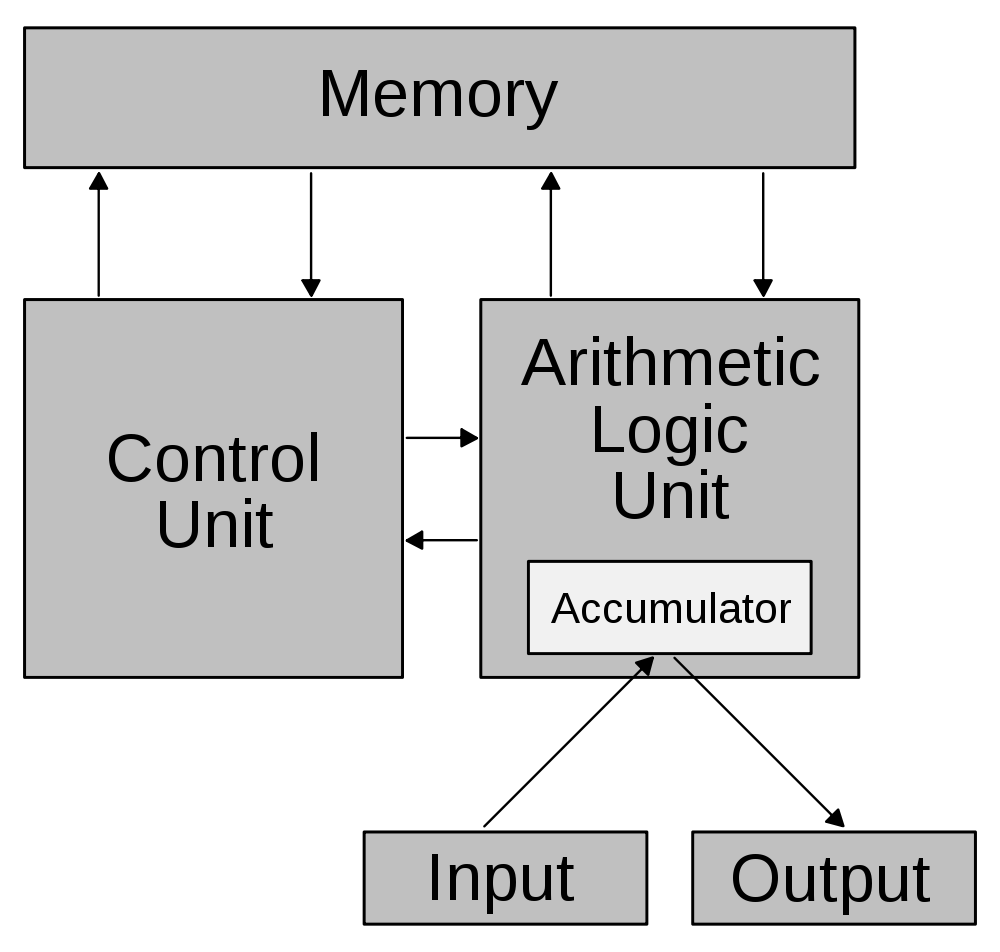
\includegraphics[width=7cm]{Von_Neumann_architecture.png}
    \caption{Schematic of the Von Neumann architecture. Wikipedia Commons}
    \label{fig:VonNeumann}
\end{figure}

some text here about von neaumann architecture

For the purpose of this thesis it is easiest to think about the architecture as three main parts, data storage, processor and the memory.

\subsection{CPU}
Central processing unit(CPU) is \cite{introduction_hpc_hager}

Until 1996 there was computers with just a single core CPU on top 500\cite{TOP500}. Since about 2005 most desktop computers CPU has several cores which has increased the need for parallel programs. The cores themselves aren't getting faster, the CPUs have more cores.

%schematic here

As you can see most of it is not used for calculations. A large part of the area is used for optimizations and caching. We will talk about caching and optimizations the next section. 

\subsection{Memory, Caching and Optimizations}
\label{optimizations}
there are various optimizations, bla bla intro
\\
Picture here of memory stuff, caching\\
\\
Retrieving data from memory is relatively slow compared to how fast the processor works\cite{introduction_hpc_hager,drepper2007cpumemory}. %TODO something about the  maginitude
To solve this problem a \emph{cache} was introduced\cite{drepper2007cpumemory}. It stores recently used data in a very small and very fast memory that resides on the CPU chip itself\cite{drepper2007cpumemory}. That data can then be reused fast without waiting for the main memory to fetch it. However when the data is not in the cache it takes the usual speed to fetch it from the main memory, that is a \emph{cache miss}\cite{drepper2007cpumemory}. Avoiding cache misses is important for speed because of how much time it can take to fetch the data from the main memory\cite{drepper2007cpumemory}. Modern CPUs commonly have more than one cache, most have three\cite{introduction_hpc_hager}. They are named L1 to L3, with L1 being the one fastest and smallest and L3 the largest and slowest\cite{introduction_hpc_hager}.\\
\\
Modern multicore processors several L1 caches, one for each core\cite{introduction_hpc_hager}. It is commonly one L2 per core too, however it is shared in some architectures\cite{introduction_hpc_hager}. L3 is almost always shared between all cores\cite{introduction_hpc_hager}. That multiple caches are used creates a problem called \emph{cache coherency}. It is that when the data is modified in one cache all the cores caches needs to be updated too so that they use the new value\cite{introduction_hpc_hager}.\\
\\
Another memory optimization somewhat related to caches is \emph{prefetching}\cite{introduction_hpc_hager, drepper2007cpumemory}. Instead of fetching just the data requested by the current operations it also fetches the surrounding data\cite{drepper2007cpumemory}. The chance that the surrounding data will be used soon is high since it is common to iterate over arrays and similar structures\cite{introduction_hpc_hager}. If a program iterates over an array unless it was used recently the first value will be a cache miss since it is not in the cache. However the following values will be due to them being prefetched and cached. At some point however the array is too long to be prefetched and cached completely and when the CPU hits that spot a new cache miss will happen\cite{drepper2007cpumemory}. Because everything is stored sequentially it is important in some cases to know how the it is stored so that the prefetching and caching can be used. One of these cases is for matrices, they are 2D but stored as one array. Different programming languages store them differently, either column by column or row by row. Row by row is called \emph{row major} and column by column is \emph{column major.}\\ %TODO cite row major and such
\\
In section 6.2.1 in What Every Programmer Should Know About Memory\cite{drepper2007cpumemory} an example of how much speed that can be gained by optimizing matrix matrix multiplication. The first version is shown in algorithm \ref{alg:matmatmult}.

\begin{algorithmCode}{Matrix matrix multiplication} {alg:matmatmult}
for (i = 0; i < N; ++i)
  for (j = 0; j< N; ++j)
    for (k = 0;k < N; ++k)
      res[i][j]+= mul1[i][k] * mul2[k][j];
\end{algorithmCode}

By transposing the mul2 matrix it becomes more cache friendly because it uses the prefectching of surrounding data the way that mul1 already is\cite{drepper2007cpumemory}. The transpose itself can be eliminated while also making it use the cache better by reading in the correct amount of data, this is the size SM in the code\cite{drepper2007cpumemory}. The optimized version is shown in \ref{alg:matmatmultopt}. It took 17.3\% of the original time\cite{drepper2007cpumemory}.

\begin{algorithmCode}{Matrix matrix multiplication optimized} {alg:matmatmultopt}
#define SM (CLS / sizeof (double))

for (i = 0; i < N; i += SM)
  for (j = 0; j < N; j += SM)
    for (k = 0; k < N; k += SM)
      for (i2 = 0, rres = &res[i][j], rmul1 = &mul1[i][k]; i2 < SM; ++i2, rres += N, rmul1 += N)
	for (k2 = 0, rmul2 = &mul2[k][j]; k2 < SM; ++k2, rmul2 += N)
	  for (j2 = 0; j2 < SM; ++j2)
	    rres[j2] += rmul1[k2] * rmul2[j2];
\end{algorithmCode}

On top of that by using some additional features of the the CPU do multiple instructions at once further speed is gained increasing it to 9.47\% of the original time\cite{drepper2007cpumemory}. \\
\\
If the operation instructions diverge, e.g. if statements, the CPU would have to wait for the results to see what instructions load and do next\cite{drepper2007cpumemory}. This can mean a lot of lost time, however thanks to a optimization called \emph{branch prediction} and \emph{speculative execution} that can be prevented in some cases\cite{drepper2007cpumemory}. A dedicated part of the CPU stores the results from these diverges and when they are repeated it uses them to make an guess of what do to next\cite{drepper2007cpumemory}. It then loads the instructions and tries to fetch the needed data\cite{drepper2007cpumemory}. It then speculatively executes the instructions, i.e it executes instructions that might not actually be needed\cite{drepper2007cpumemory}. If the guess was correct the results are kept, on the other hand if it was wrong the CPU starts again from the correct path and discards the incorrect results\cite{drepper2007cpumemory}.\\
\\
Sometimes there can be several independent instructions, e.g. when adding two vectors together, this allows optimizations for \emph{instruction level parallelism}\cite{introduction_hpc_hager}. The order of the instructions can be ignored which for instance means that if an instruction needs to wait for some data another instruction that has its data available could be executed while waiting\cite{introduction_hpc_hager}. It is an optimization called \emph{out of order execution}\cite{introduction_hpc_hager}. There are also other possible optimizations\cite{introduction_hpc_hager}.
\\
In the example \ref{ex:independent_instructions} the instructions are independent because they use different variables so they can be executed in any order. If the variables $b$ and $c$ needs to be fetched but $e$ and $f$ are available due to previous instructions then the CPU could execute the second addition first by using out of order execution. However if an operation later depends on the variable $a$ or $d$ then that instruction would have to wait until the additions have been executed.

\begin{example}{Independent Instructions}{ex:independent_instructions}
a = b + c;
d = e + f;
\end{example}

\emph{Pointer aliasing} can prevent the compiler from making certain optimizations, e.g. out of order execution mentioned above. Pointer aliasing is when the same memory area can be accessed using different variables\cite{introduction_hpc_hager}. This becomes a problem if an set of instructions use these variables in the same area of the program. The relative order of operations between these operations then has to be preserved. The compiler does have the information if aliasing occurs or not which means the compiler has to treat all situations where it can occur as if it does\cite{introduction_hpc_hager}.\\
\\
If the integers in example \ref{ex:independent_instructions} are changed to pointers then aliasing can occur because some of these pointers could point to the same memory. For instance if a and e points to the same memory then the result would be wrong if the second line is executed before the first. This would force the instructions to be executed in order or the result would likely be incorrect.

\begin{example}{Pointer Aliasing}{ex:aliasing}
//All variables are pointers
*a = *b + *c;
*d = *e + *f;
\end{example}

Some programming languages, e.g. Fortran, disallow some types of aliasing while others, e.g. C/C++, allows aliasing\cite{introduction_hpc_hager}. The compilers for the languages in the second case commonly have an option to disable aliasing. However for languages that don't allow aliasing, or if it is disabled, it is then the programmers responsibility to make sure that aliasing does not occur or the results can be wrong\cite{introduction_hpc_hager}.

\subsection{Concurrency and Threads}
\label{concurrency}
\emph{Concurrency} means doing multiple things and the same time, instead of \emph{sequential}. This can cause various problems such as the same object being accessed at the same time. The dinning philosophers is an concurrency problem that can used to illustrate some of these problems. A group of philosophers is sitting at a round table, each has a plate of spaghetti in front of them and there is a fork between each pair of philosophers\cite{hoare1985communicating}. The philosophers alternate between thinking and eating. However they can only eat if they have both the right and left fork\cite{hoare1985communicating}.

\begin{figure}[h]
    \centering
    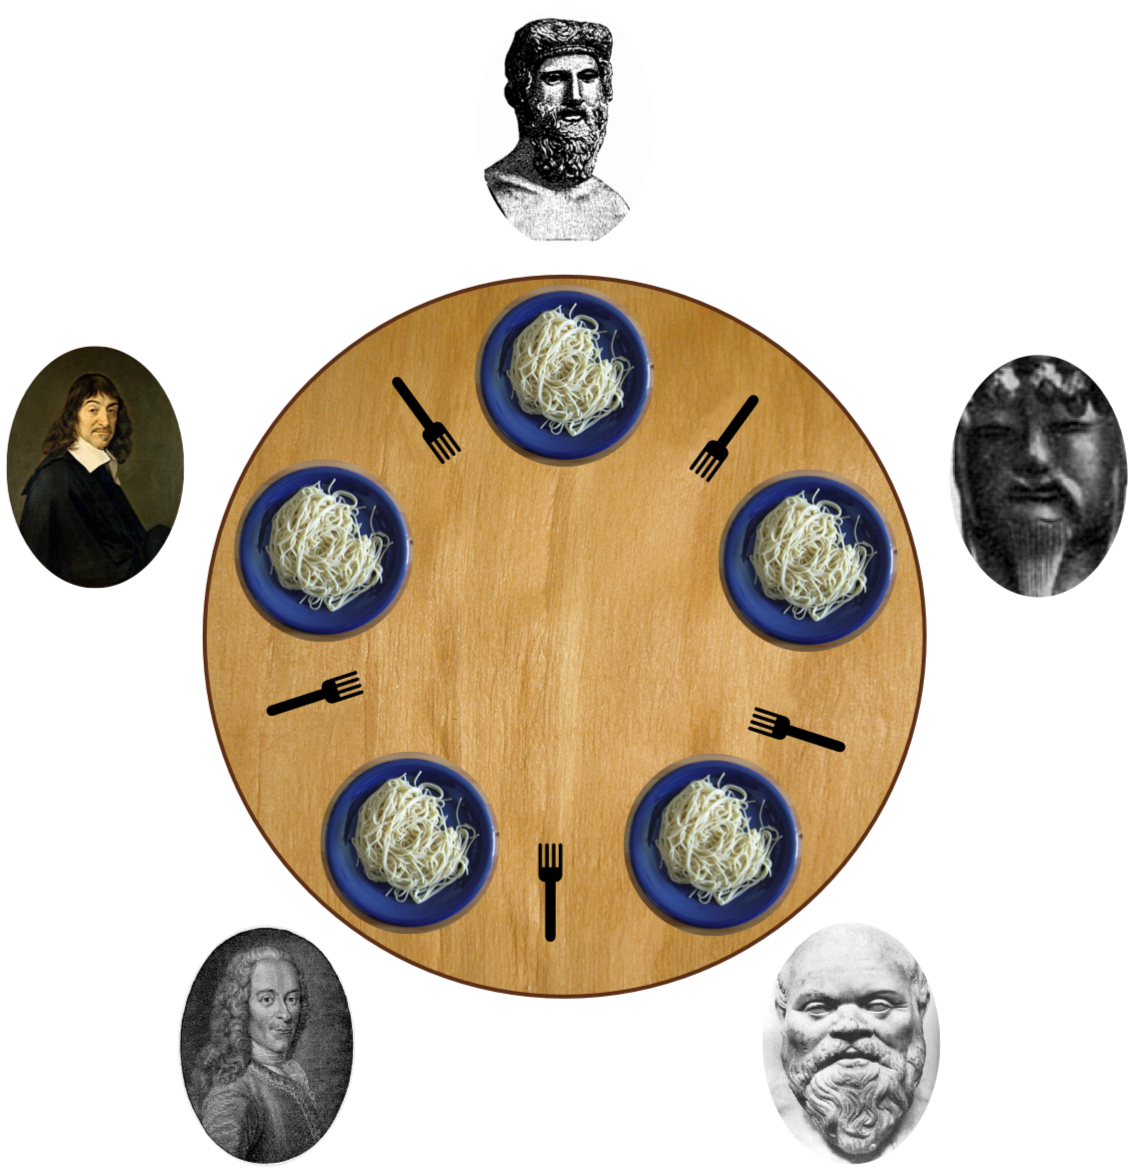
\includegraphics[width=5cm]{dining_philosophers.png}
    \caption{Illustration of the dining philosophers problem. Wikipedia Commons}
    \label{fig:dining_philosophers}
\end{figure}

A potential proposal for behaviour instructions could be:
\begin{itemize}
 \item Think
 \item Wait for a fork to become available and pick up that fork
 \item Wait for and pick up the other fork
 \item Eat
 \item Put down the forks one by one
 \item Go back to thinking
\end{itemize}
The problem is that this set of instructions can lead to a state where everyone is holding one fork and waiting to get the other one\cite{hoare1985communicating}. But no one is done eating so no forks will become available. The system is then locked into its state, this is called a \emph{deadlock}\cite{hoare1985communicating, introduction_hpc_hager}. A potential solution to the problem in this case is to introduce a person that dictates if a philosopher is allowed to eat or not\cite{hoare1985communicating}.\\
\\
There are also other potential problems that can arise when using concurrency. A \emph{race condition} occurs when the result depends on what affects it first, it is a race between them on who can reach it first\cite{introduction_hpc_hager}. \emph{Locks} can be used to prevent situations as the ones described above by making sure only one thread at a time can access the object\cite{introduction_hpc_hager}.\\
\\
In computer science concurrency occurs when instructions are separated in different \emph{threads}. The architectures can be divided in a taxonomy with four categories including the sequential. They are illustrated in figure \ref{fig:flynn_taxonomy}.

\begin{itemize}
 \item \emph{SISD}(Single-Instruction,Single-Data) is the sequential and is as the name says, single instructions on single data\cite{introduction_hpc_hager}.
 \item \emph{SIMD}(Single-Instruction, Multiple-Data) is applying the same instruction on different data\cite{introduction_hpc_hager}. SIMD is also called vectorisation\cite{introduction_hpc_hager}.
 \item \emph{MIMD}(Multiple-Instruction, Multiple-Data) applies different instructions on different data\cite{introduction_hpc_hager}.
 \item \emph{MISD}(Multiple-Instruction, Single-Data) performs different operations at the same piece of data, this paradigm is uncommon\cite{introduction_hpc_hager, computer_arch_2003}.
\end{itemize}

\begin{figure}
        \centering
        \begin{subfigure}[b]{0.48\textwidth}
                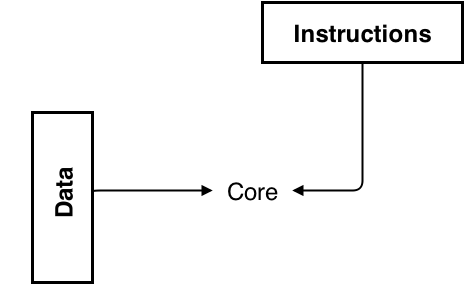
\includegraphics[width=\textwidth]{SISD}
                \caption{SISD}
                \label{fig:SISD}
        \end{subfigure}%
        ~
        \begin{subfigure}[b]{0.48\textwidth}
                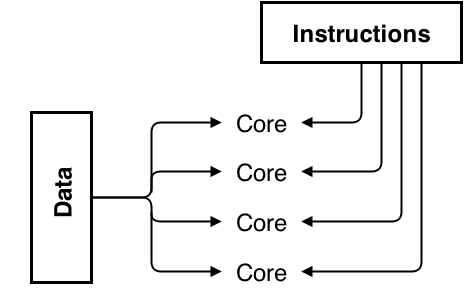
\includegraphics[width=\textwidth]{MISD}
                \caption{MISD}
                \label{fig:MISD}
        \end{subfigure}

        \begin{subfigure}[b]{0.48\textwidth}
                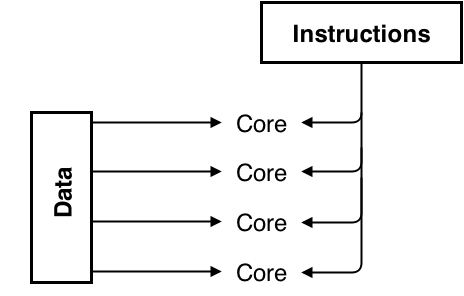
\includegraphics[width=\textwidth]{SIMD}
                \caption{SIMD}
                \label{fig:SIMD}
        \end{subfigure}
        ~
        \begin{subfigure}[b]{0.48\textwidth}
                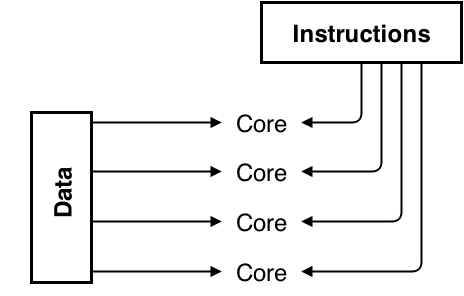
\includegraphics[width=\textwidth]{MIMD}
                \caption{MIMD}
                \label{fig:MIMD}
        \end{subfigure}
        \caption{Flynns taxonomy of parallel architectures\cite{introduction_hpc_hager}}\label{fig:flynn_taxonomy}
\end{figure}

\subsection{Accelerators, GPUs and Xeon Phi}
Graphics processing unit(GPU) have become more popular for general computing the last 10 years.

\begin{figure}[h]
    \centering
    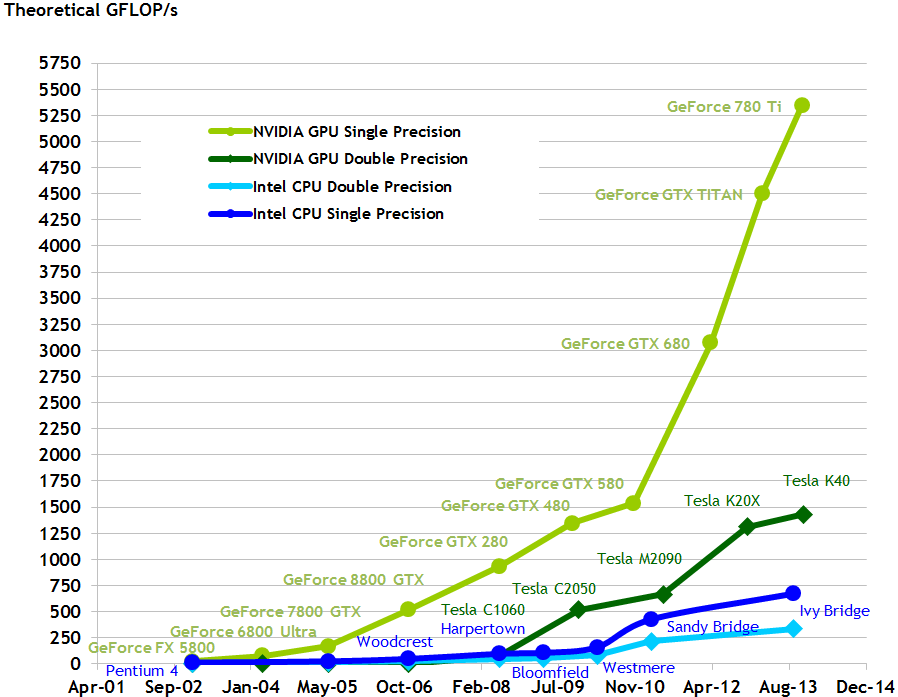
\includegraphics[width=11cm]{floating-point-operations-per-second.png}
    \caption{Bla bla \cite{cuda}}
    \label{fig:gpu_vs_cpu}
\end{figure}

%structure of gpu

'dummer' threads than CPU, more area for calculations
no branch prediction or speculative execution \ref{optimizations}


Xeon Phi, intel mic
mimd
knights landing, interesting new development from intel.
however usually but not always require memory copy
still need vectorisation and other stuff
you end up with similar problems as gpu, though probably easier to use

structure of mic

GPUs are much better at single precision calculations than double. A CPU looses some performance but not near as much as a GPU.\cite{cuda, nvtesla}

\subsection{Which program for GPU and which for CPU?}
\label{gpu_gwas}
As with a lot of things it depends on the algorithm to implement etc.

If you have lots of legacy code then then you might need to rewrite a lot. However by using a profiler the parts that take up the most time can be found and moved to the GPU. However that might be hard if the program isn't properly structured. No legacy code can also be a good thing. Old code might not be written with modern standards or use new nifty features and therefore lose speed.

Xeon Phi is an alternative, simpler but can still be tricky and have separate memory spaces.

GPUs loses more when going from single precision to double than CPUs. Peak performance on tesla-kepler cards for single precision is around 3 times higher than when using double precision\cite{nvtesla}.\\

In short GPUs excel at linear algebra but Intel MIC is probably a good alternative for it to.

GPUs are good for interaction algorithms since most approaches are embarrassingly parallel since they consider each combination independently from the others. They also often perform a lot of linear algebra. Several studies got high gains from implementing their programs on GPU, however their CPU versions weren't parallelized so it is likely that the gains would have been less compared to an optimized and parallelized CPU version.\cite{gwis,gboost,gmdr_gpu,cuda_lr,genie_2012,plink_gpu} However one study made a CPU cluster version and a GPU version of an algorithm that uses $chi^2$ tests, they found that 16 CPU nodes had the same performance as a single GTX 280 card\cite{jiang_accelerating}.

\subsection{Clusters}
%picture, server->nodes etc TODO

Clusters are collections of computers that can work together in several ways and are so tightly connected that they can usually be viewed as a single system. They communciate over a shared network but have separate memory and processors. Storage is usually shared. A computer in a cluster is called a \emph{node}. \cite{intro_hpc, kirk2012programming}

various programming models, shared memory and so on
%shared memory, cache coherrency and stuff

mpi is commonly used for clusters\cite{kirk2012programming}

top 500\cite{TOP500}

Few clusters used GPUs before 2009 but now mix of GPUs and cpu are common among the top clusters. It was driven largely by demand for power saving while still giving high performance. The GPUs can do the heavy computation while other parts are used on CPU. Most of these clusters are highly ranked in Green 500. \cite{kirk2012programming}
%Something about Intel MIC

Flops is not everything, bad performance compare to theoretical maximum
Stuck in network, hard drives, etc. Latency
Very few programs scale to the fastest clusters, peta scale.

Tianhe 2 is current top. Theoretical performance 54.9 PetaFlops.\cite{TOP500}
Max achived with LinPack 33 PetaFlops
60\% efficiency

Picture of Tianhe-2 here

\subsection{CUDA programming model}
This section is about GPU programming in more detail using NVIDIAs CUDA(Compute Unified Device Architecture)\cite{cuda}. CUDA extends C and C++ with some additional functionality that can be used to perform operations on NVIDAs GPUs. It provides a separate compiler to compile the GPU code called nvcc\cite{cuda}. Different GPUs support different CUDA functions, each NVIDIA GPU has a value called computational capability. The higher the value the more features of CUDA are supported on that GPU. Some properties also vary between the different underlying architectures. This means that it is important to know what kind of capability the GPU to be used has so that the program does not need features that are not there. The things described here might not apply to GPUs with compute capability below 3. There are GPUs made specifically for calculations rather than games. This section is an summary of how CUDA works from the CUDA programming guide\cite{cuda} and CUDA best practices guide\cite{cuda_best_practice}.\\
\\
In CUDA the GPU is called \emph{device} and systems CPU and memory is the \emph{host}. To perform operations on the device a type of function called \emph{kernel} is used. A kernel is specified the same way as a normal C/C++ function but with the addition of \_\_global\_\_ in front of the function declaration. The way the kernels are used differs slightly from normal C/C++ too. <<<...>>> is added to the it specifying how many threads to be use among others.\cite{cuda}\\
\\
Below here is an example of a kernel and how it can be called from the host code. The kernel add each element of the arrays A and B storing it in C. Each thread performs on addition and knows why elements to use based on it's id. The call to the kernel is made by giving three arrays and the number of threads to be used as N. In this case N needs to be the length of the arrays.

\begin{example}{Simple Kernel}{simple_kernel}
// Kernel definition
@__global__@ void Add(float* A, float* B, float* C)
{
  int i = threadIdx.x;
  C[i] = A[i] + B[i];
}

// In the host code
// Kernel invocation with N threads
Add@<<<1, N>>>@(A, B, C);
\end{example}

The $<<<N,M>>>$ specifier tells CUDA how many $N$ blocks and how many $M$ threads per block that the kernel should use\cite{cuda}. A block is a group of threads and shares some memory and resources. The blocks can be executed in any order so they need to be completely independent from each other but variables can be shared among threads inside a block. The blocks are  organized in a one, two or three dimensional \emph{grid}. These can be accessed by each thread so it knows which grid it is in. This can be used to make it easier to assign the threads to the correct bit of the calculation. For instance using a two dimensional grid is good for matrices\cite{cuda, cuda_best_practice}.

\begin{figure}[h]
    \centering
    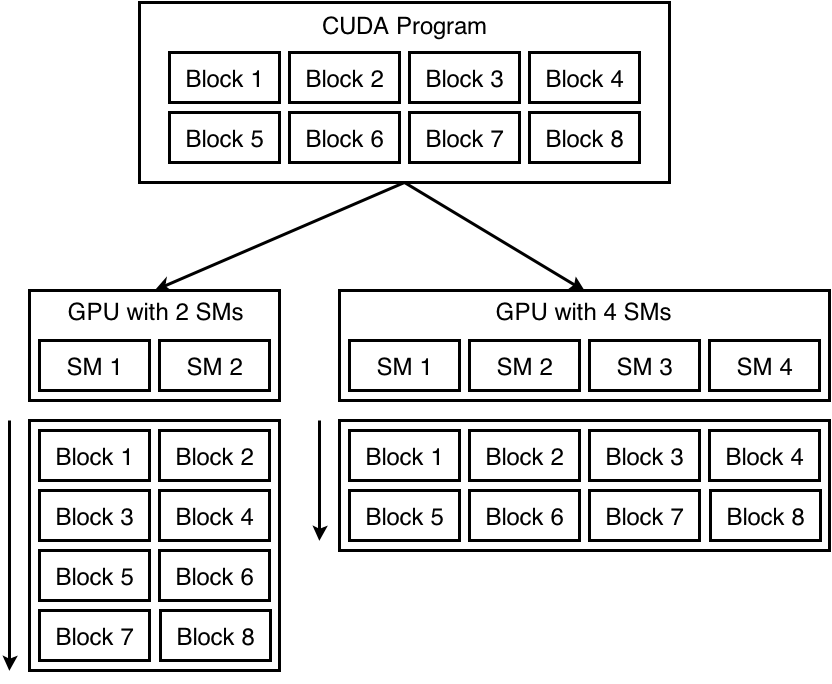
\includegraphics[width=10cm]{grid_scale.png}
    \caption{Blocks execution depending on the number of streaming multiprocessors}
    \label{fig:blocks_scaling}
\end{figure}

\begin{figure}[h]
    \centering
    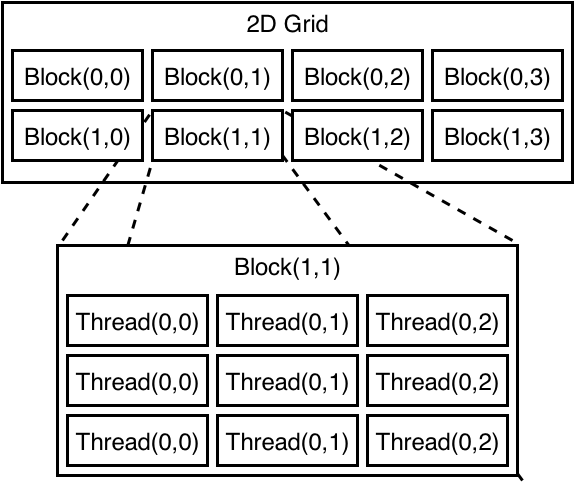
\includegraphics[width=10cm]{2D_grid.png}
    \caption{2D grid of blocks}
    \label{fig:grid_2d}
\end{figure}

The streaming multiprocessors(SM) is the hardware that handles the execution of these blocks and can execute hundreds of threads concurrently. It uses \emph{SIMT}(Single-Instruction, Multiple-Thread) which is similar to SIMD described earlier in section \ref{concurrency}. SIMT works mostly as SIMD except that it can act as MIMD on collections of threads called \emph{warps}. Each warp consists of 32 threads. When an SM gets a block it is split into warps that are assigned to warp schedulers. Each warp scheduler gives one instruction to a warp so full efficiency is achieved when all the 32 threads perform the same instruction. If there is any divergence it has to disable unrelated threads, so divergence can be costly. However different groups of warps are on different warps schedulers so can diverge without problem.\cite{cuda}

\begin{figure}[h]
    \centering
    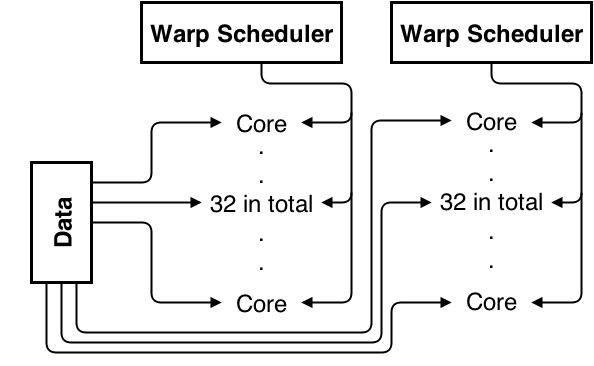
\includegraphics[width=8cm]{SIMT.png}
    \caption{SIMT architecture}
    \label{fig:SIMT}
\end{figure}

\subsubsection{Device Memory}
The GPUs memory is physically on a different device separate from the computers main memory which means that they have separate memory spaces. An object in one memory is not accessible in the other memory. The computers main memory is the \emph{host memory} and the GPUs memory is the \emph{device memory}. Since they are separate data has to be transferred to the device memory and this is done by explicit calls to transfer sections of the hosts memory.\cite{cuda}\\
\\
The GPU also have several different types of memory\cite{cuda}. Correct usage can give increased speed\cite{cuda, cuda_best_practice}.

\begin{itemize}
  \item Register memory is located on the multiprocessor and usually costs zero cycles to access. The multiprocessor splits the available registers over its threads so if there are a lot of threads that uses a lot of variables not all of them will fit in the register. This is why a program sometimes can be faster with lower number of threads.\cite{cuda}
  \item Global memory is the main memory of the GPU and is accessible from all threads and blocks. However it is relatively slow to access.\cite{cuda}
  \item Shared memory is shared inside a block and is faster than global memory. However it is limited in size.\cite{cuda}
  \item Constant memory is small however it is read only which enables some optimizations. It is best used for small variables that all threads access.\cite{cuda}
  \item Local memory is tied to the threads scope, however it still resides off-chip so it has the same access time as global memory.\cite{cuda}
  \item Texture memory is read only and can be faster to access than global memory in some situations. This was more important in older GPUs when global memory was not cached.\cite{plink_gpu, cuda}
  \item Read-only cache is available on GPUs based on Kepler architecture and uses the same cache as the texture memory. The data as to be read only each multiprocessor can have up to 48kb of space depending on GPU.\cite{kepler_tuning_guide}
\end{itemize}

\subsubsection{Streams}
\label{streams}
The kernel calls can be made on a \emph{stream}. The easiest way to think of the stream is as queue. The kernels on a stream will be executed in the order they are made but kernels from different streams can be executed in any order given there is enough computational resources. In this way it is possible to execute up to 32 concurrent kernels depending on GPU.\cite{cuda}\\
\\
This is not entirely true for some GPU architectures because they only have one queue for the kernels. Because of this independent kernels from different streams can block each other. If we have a group of kernels and issue them on stream one first and then on stream two all the kernels in stream two will be stuck in the queue waiting for the kernels in stream one to finish. This is because the kernels queue only looks at the first kernels to see if they can be executed. The second kernel in the first stream then blocks the queue from moving forward so it will not see the kernels on stream two that could be executed. Newer architectures after Kepler on the other hand has several queues so they don't have this problem.\cite{cuda, cuda_best_practice, kepler_tuning_guide}\\
\\
Streams are also important for asynchronous transfers. These transfers are executed on a stream and just as kernels gets executed after the previous kernels on the same stream is done. The advantage is that other streams can do calculations as normal while the transfer happens. This can hide the time for transfers completely in some situations as shown in \ref{fig:ascynchronous}. However the host memory has to be pinned, pinned memory means that the operative system can not page that memory. Paging is that the operative system stores a part of the memory in another area, usually the disk memory, to save space in the memory. Too much pinned memory can slow down the computer.\cite{cuda, overlap_transfers_cuda}\\
\\
However there is problem that asynchronous transfers can cause depending on the GPUs architecture\cite{overlap_transfers_cuda, cuda_fortran_overlap}. Some older GPUs only have one copy engine while newer have one for each direction, one to the GPU and one from the GPU\cite{overlap_transfers_cuda, cuda_fortran_overlap}. This can affect how the calls should be ordered and using the wrong one can make the performance worse than without using asynchronous transfers\cite{overlap_transfers_cuda, cuda_fortran_overlap}.\\
\\
There is an example of this in \cite{cuda_fortran_overlap} which illustrates the problem. They have four versions of the same code, a sequential transfer version and three asynchronous transfer versions. Two different GPUs were used, one had one copy engine the other had two. In the asynchronous the data is split over four streams coloured differently in the figure \ref{fig:ascynchronous}. Version 1 initiates the calls by looping over the streams one by one and doing the transfer and kernel calls on that stream before moving on to the next\cite{cuda_fortran_overlap}. Version 2 makes all the host to device transfer calls for all streams first, then the kernels and then the device to host transfer call\cite{cuda_fortran_overlap}. Version 3 is the same as version 2 but with a dummy even after each kernel\cite{cuda_fortran_overlap}. The figure \ref{fig:ascynchronous} shows how the transfers and kernels are executed on the GPU.

\begin{figure}[h]
    \centering
    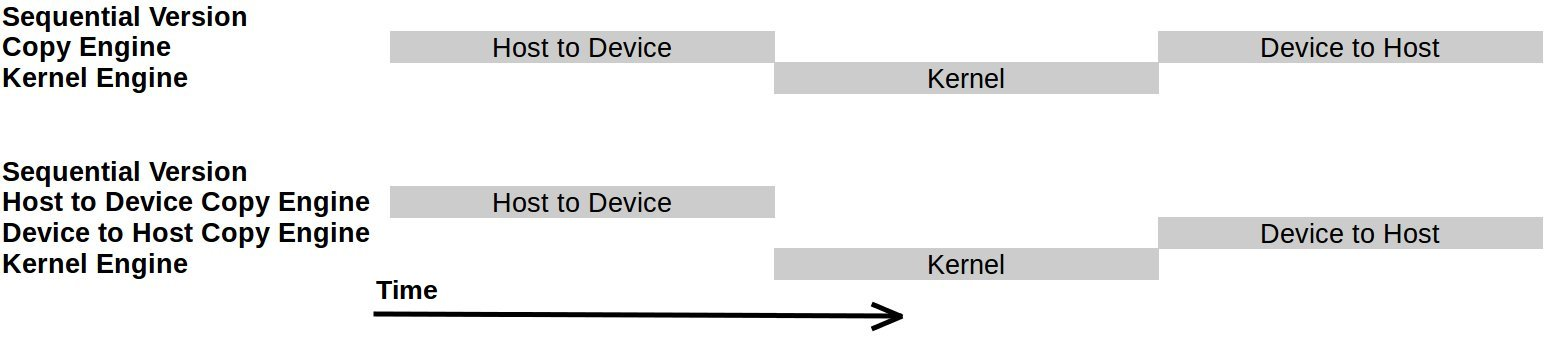
\includegraphics[width=12cm]{streams_seq.jpg}
    \caption{Sequential versions}
    \label{fig:sequential}
\end{figure}

\begin{figure}[h]
    \centering
    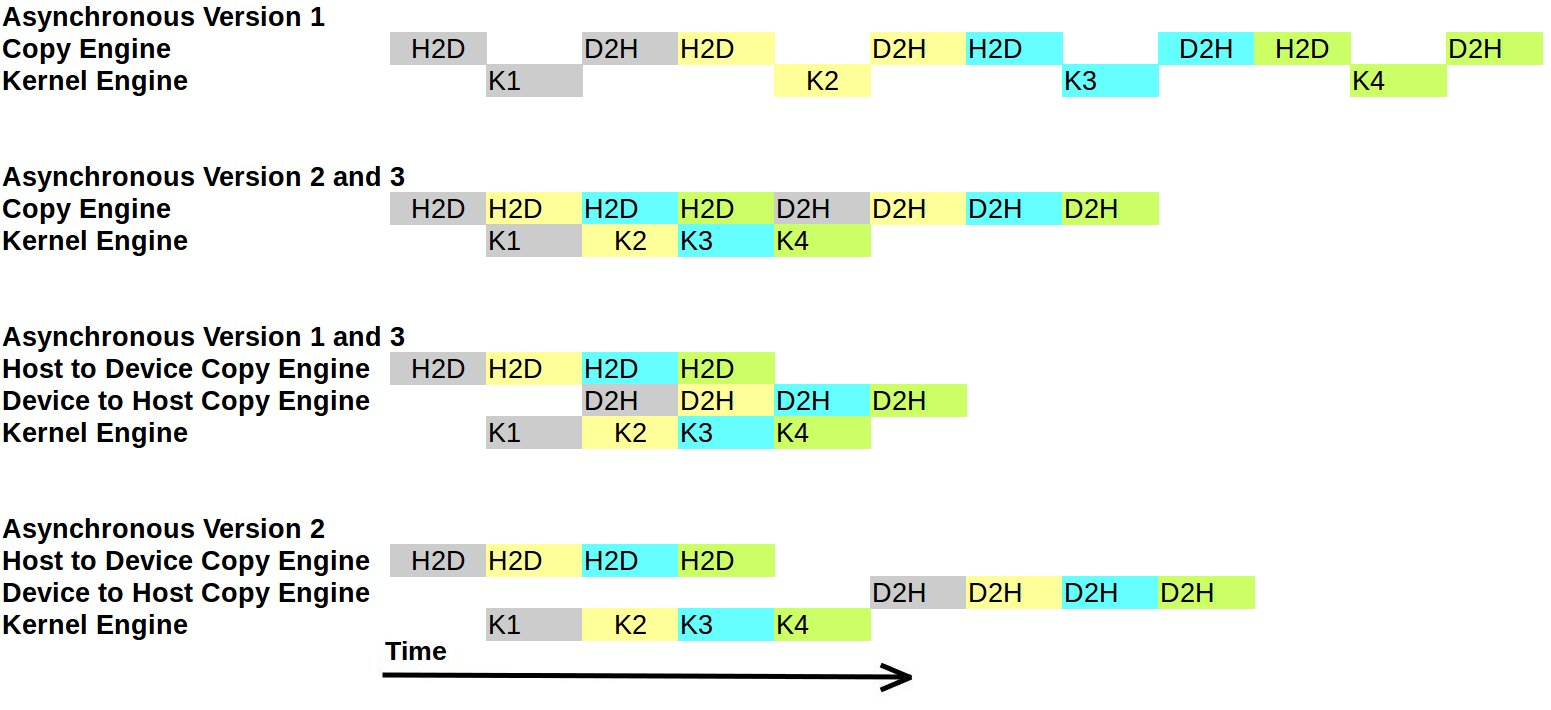
\includegraphics[width=12cm]{streams_async.jpg}
    \caption{Asynchronous versions. D2H=device to host transfer. H2D=host to device transfer. Each colour represents a stream.}
    \label{fig:ascynchronous}
\end{figure}

\subsubsection{Efficient CUDA}
One of the main criticism against GPUs for general computing purposes is that it is hard to get good performance because it requires good knowledge about details of the GPU architecture, especially the memory architecture. This section is a summary of things that can be good to consider for CUDA programs from the CUDA programming guide\cite{cuda}, CUDA best practices guide \cite{cuda_best_practice} and a similar list as this one, however slightly outdated now since it is from 2010, from a master thesis about GPU in GWAS\cite{plink_gpu}.
\\
\begin{description}
  \item[Maximize parallelism] \hfill \\
  Structure the program and the algorithm in such a way that it is as parallel as possible and overlap the serial parts on CPU with calculations on the GPU.\cite{plink_gpu, cuda}
  \item[Minimize transfers between host and device] \hfill \\
  Moving data between host and device is expensive and should be avoided if possible. It can be better to run serial parts on the GPU rather than moving the data to the host to do the calculation on the CPU. The bandwidth between host and device is one of the large performance bottlenecks. This can be a problem when the data is to large to fit in the relatively small GPU dram.\cite{cuda, cuda_best_practice}
  \item[Find the optimal number of blocks and threads] \hfill \\
  There are a lot of things affected by the number of blocks and threads so they should be considered carefully. It is a good idea to parametrize them so that they can be changed for future hardware and varied for optimization. NVIDIA has an occupancy calculator which can be helpful in determining the optimal numbers, however high occupancy does not mean high performance.\cite{cuda, cuda_best_practice}\\
  \\
  The number of blocks should be larger than the number of multiprocessors so that all multiprocessors have at least one block to execute. Having two blocks or more per multiprocessor can be good so that there are blocks that aren't waiting for a \_\_syncthreads() that can be executed. However this is not always possible due to shared memory usage and similar.\cite{cuda_best_practice}\\
  \\  
  The number of threads per block should be a multiplier of 32 but minimum 64. It's also important to remember that multiple concurrent blocks can reside on the same multiprocessor. Too large number of threads in a block and parts of the multiprocessor might be idle since there aren't a block small enough to use those threads. Between 128 and 256 threads is a good place to start.\cite{cuda_best_practice}
  \item[Use streams and asynchronous transfers] \hfill \\
  By using streams it is possible to overlap memory transfers with calculations as mentioned before. This means that the data for the next batch can be transferred while the current batch is calculated and when it is done it can start calculating on the next batch directly after the current one is done. This can hide the time for transfers completely in some situations. Depending on the time the transfers take versus the time the calculations take this can give significant speedup.\cite{cuda, overlap_transfers_cuda, kepler_tuning_guide}
  \item[Use the correct memory type and caches] \hfill \\
  Correct use of caches and memory is important for both CPU\cite{drepper2007cpumemory} and GPU. However it is more complicated on GPU since the caches are smaller and there are several types of memory as mentioned before\cite{cuda, cuda_best_practice}.
  \item[Avoid divergence] \hfill \\
  Each thread in a warp executes the same instruction at the same time so if some of threads diverge the rest will be ideal until they are at the same instruction again. This means it is important to use control structures such as if statements carefully to prevent threads from idling.\cite{cuda, cuda_best_practice}
  \item[Avoid memory bank conflicts when using shared memory] \hfill \\
  Shared memory is divided into equally-sized memory modules called banks that can be accessed at the same time for higher bandwidth. Bank conflicts occur when separate threads access the same bank. On some GPUs it is fine if all threads access the same bank. Bank conflicts are split into as many conflict-free requests as needed.\cite{cuda, cuda_best_practice}
  \item[Use existing libraries] \hfill \\
  Instead of writing everything from scratch it is usually a good idea to use already existing libraries. Especially when performance is important and most task are non trivial on GPUs so using an already optimized library is a good idea. Some of the most popular libraries for CUDA are:
  \begin{itemize}
    \item CUBLAS: BLAS implementation for CUDA. BLAS and LAPACK is a standard for a library that provides highly optimized functions for linear algebra.\cite{cublas}
    \item CULAtools: BLAS and LAPACK implementation for CUDA for both dense and sparse matrices\cite{culatools}
    \item MAGMA: BLAS and LAPACK implementation among other things that can distribute the work on both CPU and GPU\cite{magma_2010}
    \item Thrust: Template based library that tries to emulate C++ standard library\cite{thrust_gpu}
  \end{itemize}
  \item[Avoid slow instructions] \hfill \\
  There are some instructions that can be slow and should be avoided if possible, for instance type conversion, integer division and modulo. If a function is called with a floating point number that might be used as a double and require a conversion. By putting an $f$ at the end of the number it is told to be single precision float, for instance 0.5f. In some cases it is possible to use bitwise operations instead which is faster.\cite{cuda, cuda_best_practice}
  \item[Restricted pointers can give increased performance] \hfill \\
  Aliasing can be a problem as mentioned earlier. By using the \_\_restrict\_\_ keyword on pointers the compiler can be told that no aliasing will occur, however it is up to the programmer to make sure that is the case or there might be unexpected results. Not using aliasing reduces the number of memory accesses the CPU needs to make. However it increases register pressure so it can have an negative effect on performance.\cite{cuda}
  \item[Use fast math functions if precision isn't needed] \hfill \\
  There are three versions of the math functions. The double precision version is func() while the single precision function is funcf(). There is third faster but less accurate version \_funcf(). The option -use\_fast\_math makes the compiler change all the funcf() to \_funcf().\cite{cuda_best_practice}
  \item[Instruction level parallelism can increase speed]\hfill \\
  Just as for CPUs the GPUs can take advantage of instruction level parallelism. By unrolling loops this can give 2x the speed relatively simple\cite{volkov2011unrolling}.
\end{description}

\clearpage
\subsection{Performance Measures}
An important part in making fast and efficient programs is to know how fast the program is under certain conditions and which parts of the program are slow\cite{introduction_hpc_hager}. For instance the speed could suddenly drop when we start using too many threads, there might be a bottleneck in the network, and so on.\\
\\
There are two ways to measure how long a program takes to execute\cite{introduction_hpc_hager}. Wall clock time is how long real life time the program took. The other is to measure the number of processor cycles spent. A parallel program will have shorter execution time than it is serial version however it will likely have spent more processor cycles due to overhead from communication and initialization of the threads. These two measures are useful for different kinds of comparisons. Wall clock time is better for overall performance while number of cycles is useful for comparing different algorithms\cite{introduction_hpc_hager, cuda_best_practice}.\\
\\
Speed up is a measure of how much faster then program is with a certain number of threads compared to the serial version. It's defined as\cite{introduction_hpc_hager}
$$S(p)=\frac{T(1)}{T(p)}$$
Where $T(1)$ is execution time of serial program and $T(p)$ is execution time of parallel program with p threads. Linear speed up is when S(p)=p\cite{introduction_hpc_hager}.\\
\\
Efficiency reflects how efficient the program is using p threads. Linear speed has efficiency 1. It's defined as\cite{introduction_hpc_hager}
$$E(p)=\frac{S(p)}{p}=\frac{T(1)}{pT(p)}$$
\\
Strong scaling refers to how the program handles a fixed problem size and increased number of processors\cite{introduction_hpc_hager}. An program with strong scaling has linear speed up\cite{introduction_hpc_hager}. Weak scaling refers to the execution time of the program when there is a fixed problem size \emph{per processor} and the number of processors is increased\cite{introduction_hpc_hager, cuda_best_practice}.\\
\\
It can be a good idea to plot these measures while varying p, this can show when a bottleneck occurs. Looking at the measures at node level can also be useful to get an idea of how increased number of nodes and therefore increased communication over the network affects the performance.

\subsubsection{Amdahl's Law and Gustafson's Law}
Amdahl's Law is used to find the expected speed up of a system when parts of it are made concurrent. Simply it says that as the number of processors increases the parts that aren't parallel will start taking up more and more of the wall clock time and that the speed up for adding more processors will decrease as more and more processors are added and more time is spent relatively on the non parallel parts\cite{introduction_hpc_hager}. It's closely related to strong scaling.\cite{cuda_best_practice,2010_reevaluating_amdahl}\\
\\
It says that the expected speed up with F fraction of the code parallel and p threads is\cite{introduction_hpc_hager} 
$$S(p)=\frac{1}{(1-F)+\frac{F}{p}(1-F)}$$
As the number of threads grow towards infinity $S(p)$ converges on $\frac{1}{1-F}$. If we have 90\% of a code parallel then even with infinite number of threads we won't get a better speed up than ten.\cite{2010_reevaluating_amdahl}

\begin{figure}[h]
    \centering
    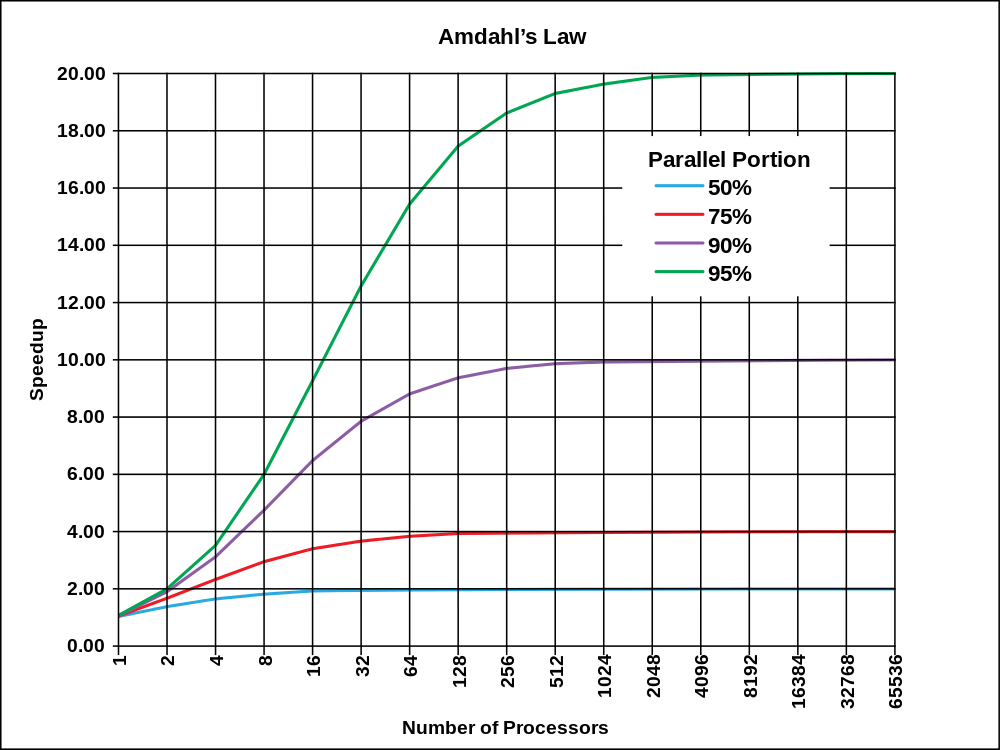
\includegraphics[width=11cm]{AmdahlsLaw.png}
    \caption{Illustration of Amdahl's Law. Wikipedia Commons}
    \label{fig:AmdahlsLaw}
\end{figure}

There are limitation to Amdahl's Law since it makes a couple of assumptions.

\begin{itemize}
  \item The number of executing threads remain constant over the course of the program.
  \item The parallel portion has perfect speed up. Often not true due to shared resources,eg caches, memory bandwidth, and shared data.
  \item The parallel portion has infinite scaling, not true due to similar limits as above. More threads will not increase performance after a while or might even decrease it.
  \item There is no overhead for creation and destruction of threads.
  \item The length of the serial portion is independent of the number of threads. Often the serial work is to divided the work to the threads, this work will obviously increase as the number of threads go up. More threads can also lead to more communication overhead.
  \item The serial portion can't be overlapped by the parallel parts. For instance with producer consumer type pattern the consumer could be strictly serial but the time it takes could be overlapped by the parallel producers.
\end{itemize}

This means it is most accurate with programs that are of the fork-join type, e.g. both serial and parallel parts\cite{gustafson1988reevaluating}.\\
\\
Gustafson's Law is closely related to Amdahl's Law and can in some ways be more accurate than Amdahl's Law\cite{gustafson1988reevaluating}. Gustafson's Law makes similar assumptions as Amdahl's Law however it also makes two additional statements. It states that problems tends to expand when provided with more computational power, e.g. increased precision by reducing grid size for simulations, higher frame rate for graphics and so on\cite{gustafson1988reevaluating, introduction_hpc_hager}. The second is that the parallel portion of the program tends to expand faster than the serial part, e.g. for matrix multiplication the initialization scales linearly with the matrix size while the multiplication itself scales as $O(n^3)$\cite{gustafson1988reevaluating, introduction_hpc_hager}. The former means that it is closely related to weak scaling\cite{introduction_hpc_hager}. So in a way it says that the execution time remains constant rather than the amount of data. More precise it says that the expected speed up with p threads and F fraction of the code that is parallel is\cite{gustafson1988reevaluating, cuda_best_practice, introduction_hpc_hager}
$$S(p)=p+(1-F)(1-p)$$

\begin{figure}[h]
    \centering
    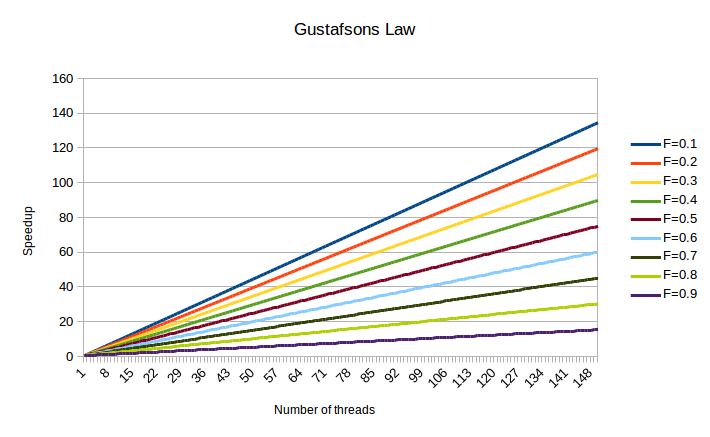
\includegraphics[width=13cm]{GustafsonsLaw.png}
    \caption{Illustration of Gustafson's Law}
    \label{fig:GustafsonsLaw}
\end{figure}

\subsubsection{Profilers}
There are applications called profilers that are made to assess the programs performance and resource consumption. They calculate some of the measures mentioned earlier and they also check hardware usage and how much time the program spends at various parts of the program. This is very useful for finding bottlenecks and other problems in the program. It does not matter if the algorithm is super fast if all the data is stuck in network transfers. The profilers can be hardware dependent so the manufactures usually provided them for their products.\cite{introduction_hpc_hager, cuda_best_practice}

%TODO lite om nsight

\clearpage
\section{Software Design}
How to design software so it can be maintained over time has been a problem for a long time. Object oriented languages such as C and later Java and C++ arose because of problems with maintaining software. Badly organized and written code will cost productivity in the future when bugs and other problems stack up because of earlier mistakes. Fixing those bugs are likely to time consuming because it can be hard to find where they originated from. All code gather problems overtime, however a well designed system will degenerate a lot slower than one that was designed carelessly. The code will also be read by ourselves and others later which means readability is important if a future reader is to understand the code and find the parts they are interested in. \cite{cleancode2008, design_patterns}\\
\\
This is also important in science where others might wish to use the tools or repeat the experiments. A recent study\cite{comp_repro_2013} found that the repeatability in computer science is low. They used the term reproducibility however repeatability is a more fitting term because they didn't try to reproduce the results from scratch, they tried to repeat it using the same code. Of 513 articles they received the code from 231, 108 failed to build, 21 failed to run properly\cite{comp_repro_2013}. Just 102 worked properly\cite{comp_repro_2013}.\\
\\
There are ways to design the program and code in such a way that it is easier to read and maintain. Most of the things described here goes under the development technique called agile development and the concept of clean code and is a summary of some concepts from the book Clean Code\cite{cleancode2008}. SOLID is an acronym for five principles for object oriented programming and design\cite{cleancode2008}. When used together they are intended to make programs that are easy to maintain and extend. As already mentioned readability is important. Correct names will make the code explain itself without other documentation, the code itself is the documentation.

\begin{table}[h]
\begin{tabular}{ l l p{2in}}
  \hline
  Initial & Principal & Concept\\
  \hline
  S & Single responsibility principle & A class should only have a single responsibility \\
  O & Open/closed principle & A class should be open for extension but closed for modification \\
  L & Liskov substitution principle & If S is a subtype of T, then objects of type T may be replaced by objects of type S without without altering any of the desirable properties of the program(e.g. work performed)\\
  I & Interface segregation principle & Use several smaller and more specific interfaces instead of one large \\
  D & Dependency inversion principle & Depend on abstractions(e.g. interfaces) not details \\
  \hline  
\end{tabular}
\caption{The five SOLID principles, from \cite{cleancode2008}}
\label{table:solid_table}
\end{table}

Dependency injection is one way to implement dependency inversion principle\cite{cleancode2008}. Injection is passing the dependency to the dependent object. This is used instead of allowing the dependent object to construct or find the dependency.

\subsection{Unit Tests and Mocks}
\emph{Unit testing} involves testing the program in small units in isolation. Testing in isolation means that the test should only depend on the part of the program that is tested. If a part of the program is not working properly only its related tests should fail, not other tests for code that depends on it but otherwise works properly. This makes it easier to find errors when they do occur since the tests will pinpoint the unit which does not work.\cite{cleancode2008}\\
\\
It can be easy to denote test code as less important than the main code but they should be treated as equally important. Tests should also not be an inconvenience to use so they should be easy to run, take reasonable amount of time to complete and not require any outside interpretation whether they failed or not.\cite{cleancode2008}\\
\\
\emph{Mocking} is to replace a real object with a fake object called a \emph{mock} that for the code is indistinguishable from the real object. This allows one to create situations and test with more control and without depending on the real objects code. The second is important for unit tests since it enables one to test units that normally depend on others in isolation. In the first case it is useful in situations such as when one wants to test a class handling of a rare failure. Such failures can be hard and time consuming to induce. It is then easier to use a mock object that behaves like the failure has occurred. However mocking requires that the code for the class doesn't create the object itself since there is no way to replace the object with the mock. This is one of the reasons why dependency injection should be use.\cite{cleancode2008}

\subsection{Design Patterns}
\label{design_pattern}
A \emph{design pattern} in software design is a reusable general solution to a common recurring problem in a given context. It is templates and structures to solve the problem, however it is not code. However they are partially dependent on the programming language since different languages have different features and limitations.\cite{design_patterns}\\
\\
\emph{Consumer producer} is a concurrency pattern for when there are a number of consumers/workers and producers. They share a common queue for products. The producer generates some product and put it into the queue, while the the consumers consume the products. The problem is that the producers should not add to an non empty slot and that each product should only be consumed once.\cite{cleancode2008, design_patterns}

\subsection{Version Control Software}
%TODO

For this project git was used and the code can be found at \url{https://github.com/Berjiz/CuEira}

git
cite git

\clearpage
\chapter{Algorithm}
%Algorithm (up till 20 pages)
%  - Current state - Basic algorithm, Data structure, memory consumption, parallelization, load balancing and scalability
%  - And the same for own your implementation

%TODO nån typ av intro här

%OTHERS
%problem with exathsutive

%memory problems(GENIE, CUDALR and so on), possibly JEIRA/GEISA

%2 bit 3 bit data storage

%two stage analysis

plink data format

\section{Current algorithm, JEIRA and GEISA}
JEIRA and GEISA uses Java and its built-in functions for concurrency. Since GEISA is based on JEIRA, as talked about in section \ref{jeira}, they both work in roughly the same way.\\
\\
The implementation uses the producer consumer pattern described in section \ref{design_pattern}. The main thread creates a queue of tasks. All the result producers iterates over this shared queue and outputs results. These results are placed in a queue a consumed by another thread that prints the results. The program reads all data at the start which means it can get memory problems for large datasets.

%risk allele diff

%strucuture picture

\section{CuEira}

%structure picture

why lr
-less sever drawbakcs for non binary
-can handle non binary data(however statistical problems needs to be solved)
-slow but is not too slow for gene-environment interaction

Dependencies
-boost
-cmake+make
-mkl
-intel compiler
-google test and mock, already included in the source due to easier compiling

C++ is row major but this program is column major completely. Because BLAS and CUBLAS

In the initialisation step it reads all the data except the information for the individuals in the SNPs, i.e. it doesn't read the bed file at that stage.
Shared blocking queue and a result writer
3 threads per GPU
Each thread has one CUDA stream
Each thread gets a snp from the queue, reads in the snp data, calculates the models and writes the results

Outcomes shared over whole GPU

LR
Some parts on GPU, some parts on CPU
Which parts?
Why?

%optimizations
%compilers

\chapter{Results}
%Results (up till 15 pages including plots)
%  - Performance measurements (scalability, speed up and efficiency as well as load balancing)
%  - Setup(simulation setup, compilers and hardware setup)
%  - Single node performance
%  - multy-node performance


%What was used
%Zorn specs
%compiler intel 14.0
%cmake 2.8
%mkl 13.1
%cuda 5.5

single vs double precision

fast math

no aliasing

kepler vs fermi queue problem, problem described in section \ref{streams}

personHandler is slow

\chapter{Discussion and Conclusions}
%Discussion and Conclusions (up to 3 pages)
%Need for novel methods for gene-environment interaction
%Need for methods for third order interaction and higher
%more statistics for non binary

%TODO look back att efficent cuda part

%TODO divergence problems, nothing now but could be with recoding on GPU or bootstrap
%idea for solution using pointer architmic

\chapter{Outlook}
%Outlook (up to one page)
more statistics for non binary

need to change mkl to any blas and remove dependency on intel compiler

clusters
kinda possible by splitting the input files

cublas not that much harder than regular blas. A wrapper could enable simple and easy use without losing too much features.
own kernels more than simple elemntwise, probably hard to optimize. unknowish

\chapter{Appendix}
\section{List of Variables}

\begin{description}
%anything with hat is estimate
\item[$\theta_{ij}$]
  Odds ratio with exposure levels i and j
\item[$RR_{ij}$]
  Relative risk with exposure levels i and j
\item[X]
  Predictors
\item[Y]
  The outcome, binary variable
\item[$\pi(x)$]
  = $P(Y=1)$
\item[$\Omega$]
  Odds
\end{description}

\section{List of Abbreviations}

\begin{description}
\item[MAF] \hfill \\
  Minor allele frequency, the frequency of the least common allele.
\item[RF] \hfill \\
  Random Forest
  MDR
  OR
  RR
  RERI
  AP
  SI
  GPU
  CPU
  CUDA
  RR
  streaming multiprocessors(SM)
  SIMD
  SIMT
  MIMD
  SISD
  MISD
  LR
\end{description}

\section{Environmental and Covariates File Format}
The environmental factors and covariates are stored in separate files with the same format, one file for environmental factors and one for the covariates if any. One of the columns needs to contain the individual ids, the rest of the columns should be data. The delimiter can be anything of the usual ones and there is an option to provided it to the program. The default is tab delimited.

%List of figs
%List of tables


\newpage
\bibliographystyle{ieeetr}
\bibliography{hpc.bib,statistics.bib,misc.bib}
\end{document}